\synctex=1
\documentclass[12pt,a4paper,oneside]{article}

\usepackage[spanish]{babel}

\usepackage{fancyhdr}
\usepackage{geometry}
\usepackage{graphicx}
\usepackage{wrapfig}
\usepackage{lastpage}
\usepackage[hidelinks]{hyperref}
\usepackage{authblk}
\usepackage{bookmark}

\usepackage[utf8]{inputenc} % Required for inputting international characters
\usepackage[T1]{fontenc} % Output font encoding for international characters
\usepackage{mathpazo} % Palatino font

\makeatletter
\newcommand{\subtitledoc}[1]{\newcommand{\@subtitledoc}{#1}}
\newcommand{\instituto}[1]{\newcommand{\@instituto}{#1}}
\newcommand{\carrera}[1]{\newcommand{\@carrera}{#1}}
\newcommand{\professor}[1]{\newcommand{\@professor}{#1}}
\newcommand{\catedraCaratula}[1]{\newcommand{\@catedraCaratula}{#1}}
\newcommand{\catedraHeader}[1]{\newcommand{\@catedraHeader}{#1}}
\newcommand{\curso}[1]{\newcommand{\@curso}{#1}}
\newcommand{\legajo}[1]{\newcommand{\@legajo}{#1}}
\newcommand{\footerauthor}[1]{\newcommand{\@footerauthor}{#1}}
\newcommand{\footerlegajo}[1]{\newcommand{\@footerlegajo}{#1}}

%Configuracion de hoja (margenes y tamaño)
\geometry{a4paper,margin=1in}
\setlength\headheight{28pt}

%formato de encabezado y pie para todas las paginas.
\fancyhead[L]{
    \begin{minipage}[b]{7.5mm}
        
\includegraphics[width=7mm]{Imagenes/logo-utn.png}
    \end{minipage}
    \begin{minipage}[b]{90mm}
        \textbf{Alumnos: }\@footerauthor \\
        \textbf{Legajos: }\@footerlegajo
    \end{minipage}
}
\fancyhead[R]{
    \textbf{Curso:} \@curso\\
    \textbf{Cátedra:} \@catedraHeader
}
\fancyfoot[L]{\@date}
\fancyfoot[C]{} %eliminar antiguo numero de pagina
\fancyfoot[R]{Página \thepage\ de \pageref{LastPage}}
\renewcommand{\headrulewidth}{0.5pt}
\renewcommand{\footrulewidth}{0.5pt}
\pagestyle{fancy}

\addto\captionsspanish{%
	\renewcommand{\contentsname}%
	{CONTENIDO}%
}

\renewcommand{\maketitle}{%
    \newpage
    \thispagestyle{empty}
    
    \begin{center}

    \textsc{\LARGE \@instituto}\\[0.5cm] 
    \textsc{\Large \@carrera}\\[1.5cm] 
    
\includegraphics[width=0.30\textwidth]{Imagenes/logo-utn.png} \par
    \vspace{1.5cm}
    
    \textsc{\large \@catedraCaratula }\\[0.5cm]
    
    {\huge\bfseries \@title}\\[0.4cm]
    \textsc{\Large \@subtitledoc}\\[0.5cm]
    

    \end{center}

    \vspace{2cm}

    {\noindent
    \begin{minipage}[t]{.2\textwidth}
        \raggedright
        \textbf{ALUMNOS} \par
        ~\\
        ~\\
        ~\\
        \textbf{CURSO} \par
        ~\\
        \textbf{DOCENTES} \par
        \end{minipage}%
     \begin{minipage}[t]{.05\textwidth}
        \raggedright
        \textbf{:} \par
        ~\\
        ~\\
        ~\\
        \textbf{:} \par
        ~\\
        \textbf{:} \par
    \end{minipage}%
    \begin{minipage}[t]{.55\textwidth}
        \raggedright
        \@author \par
        ~\\
        \@curso \par
        ~\\
        \@professor \par
        ~\\
    \end{minipage}%
    \begin{minipage}[t]{.15\textwidth}
        \raggedright
        \@legajo \par
    \end{minipage}
    }
    \vfill
    \begin{center}
        \textbf{CÓRDOBA, ARGENTINA} \par
        \textbf{\@date}
    \end{center}
    \newpage
}

\makeatother


\instituto{Universidad Tecnológica Nacional\\[0.2cm]Facultad Regional Córdoba}
\carrera{Ingeniería Electrónica}
\title{Trabajo Práctico de Laboratorio Nº11}
\subtitledoc{Análisis de señales con osciloscopios digitales}
\professor{Ing. Centeno, Carlos \par Ing. Salamero, Martin \par Ing. Guanuco, Luis}
\catedraCaratula{Medidas Electrónicas I}
\catedraHeader{Med. Electrónicas I}
\curso{4R1}
\author{Carreño Marin, Sebastian \par Juarez, Daniel \par Torres, Heber}
\legajo{83497 \par 79111 \par 84640}
\footerauthor{Carreño Marin, Juarez, Torres}
\footerlegajo{83497, 79111, 84640}
%\date{\the\year}
\date{6 de octubre de 2022}



\usepackage{float} %Mejora la interfaz para definir objetos flotantes
\usepackage{caption} %Permite customizar captions en entornos flotantes como figuras y tablas
\usepackage{subcaption} %Provee lo mismo que captions pero para subfiguras y similares

\usepackage{amsmath} %Paquete matemático
\usepackage{amssymb} %Provee flechas, operadores, caracteres especiales, figuras geométricas, etc.
\usepackage{mathtools} %Provee una serie de paquetes que mejoran la apariencia de documentos con matemáticas. Basado en amsmath
\usepackage{siunitx} %Unidades del Sistema Internacional

\usepackage{booktabs} %Mejora la calidad de las tablas
\usepackage{multirow} 
\usepackage{multicol}
\usepackage{array} %Implementación extendida de los entornos array y tabular

\usepackage{enumerate} %Agrega un argumento opcional al entonrno enumerate

\usepackage{soul} %Proporciona espaciado separable con guiones, subrayado, tachado, etc.

%\usepackage{svg} %Permite la integración de gráficos SVG
%\usepackage{blindtext} %Provee comandos para crear textos 'blind' utiles para testear clases y paquetes

\usepackage[spanish]{babel} \addto\captionsspanish{\def\tablename{Tabla}   
\def\listtablename{\'Indice de tablas} } 



\begin{document}
  \maketitle

  \null
  \thispagestyle{empty}
  \pagebreak

  \setcounter{page}{1}
  \tableofcontents
  \newpage
  %\listoffigures
  %\listoftables
  %\pagebreak
  
    \section{Introducción}
    Algunos osciloscopios digitales poseen un módulo matemático, el cual incluye la
    \textit{Transformada Rápida de Fourier} (FFT). Esta herramienta permite analizar
    señales en el dominio de la frecuencia, lo cual es útil en determinadas ocasiones.
    Por otro lado, estos osciloscopios otorgan utilidades en los menú de medidas, que
    permiten caracterizar de forma rápida la señal en cuestión. Todos
    estos detalles son tratados en el presente informe.

    \section{Marco Teórico}

    Realizar análisis de señales en dominio de la frecuencia, posee la ventaja de poder 
    brindar mas información a diferencia de hacerlo bajo el dominio del tiempo. 
    Por ejemplo, se puede visualizar una onda senoidal en el tiempo ,entregada 
    por un generador de funciones, con un osciloscopio y notar una distorsión muy leve 
    en sus picos, casi imperceptible, lo cual, si dicha señal se la analizara bajo el 
    dominio de la frecuencia, quedaria en evidencia clara que la misma no es una señal 
    senoidal pura sino que posee armónicos debido al modo que utilizan los generadodes 
    de funciones para crear dicha señal.
    
    La desventaja de analizar señales en el 
    dominio de la frecuencia es que no se puede obtener información de la fase relativa de 
    la señal bajo análisis, solo es posible obtener la amplitud de las componentes
    espectrales. La otra desventaja a destacar es que, resulta difícil realizar análisis de 
    transitorios rapidos, estos mismos son mas comodos de analizar en el dominio del tiempo.
    
    Para el presente trabajo practico se realizará los ensayos con un osciloscopio digital 
    el cual posee un modulo matemático (\textbf{Math menu}) que cuenta con la transformada 
    rapida de Fourier (FFT). 

    \subsubsection{Analizador de Fourier }
    
    El analizador de fourier, posee un conjunto de filtros donde cada uno de los 
    mismos se encuentran ligeramente desfasados entre si y repartidos de manera 
    uniforme sobre el margen de frecuencia que se desea analizar, tal como se observa
    en la Figura~\ref{fig:EsqInicialFourier}. El conjunto de filtros puede formar 
    parte de un sistema mas complejo, donde sus salidas pueden ser multiplexadas 
    y mostradas en conjunto con un amplificador vertical en una pantalla y a su ves, 
    el multiplexor con un contador, aparte de seleccionar el conjunto de filtros, 
    generar una señal de rampa escalera para posteriormente pasar por un 
    amplificador horizontal y realizar un barrio de eje horizontal de la pantalla 
    para poder visualizar el espectro en frecuencia de una señal. En la 
    Figura~\ref{fig:EsqAnalizadorDeFourierBasico}, se muestra un diagrama en bloques 
    simplificado de un analizador de fourier el cual, su principal 
    ventaja es que, el análisis se hace practicamente en forma simultánea en todo 
    el espectro. Pero dichos instrumentos poseen como desventaja una excesiva 
    complejidad del sistema y a su vez poseen baja resolución con un \textit{spam} 
    (margen de frecuencia de trabajo) fijo.
    \begin{figure}[H]
        \centering
        \begin{subfigure}[H]{0.48\textwidth}
          \frame{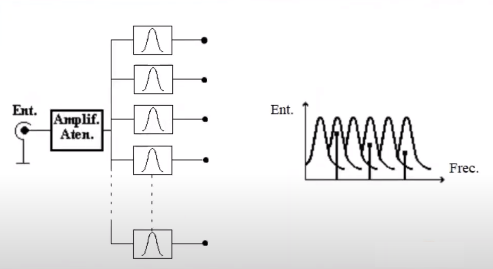
\includegraphics[width=\textwidth]{Imagenes/MarcoTeorico/EsqInicialAnalizDeFourier.png}}
          \caption{Conjunto de Filtros.}
          \label{fig:EsqInicialFourier}
        \end{subfigure}
        \hfill 
        \begin{subfigure}[H]{0.45\textwidth}
          \frame{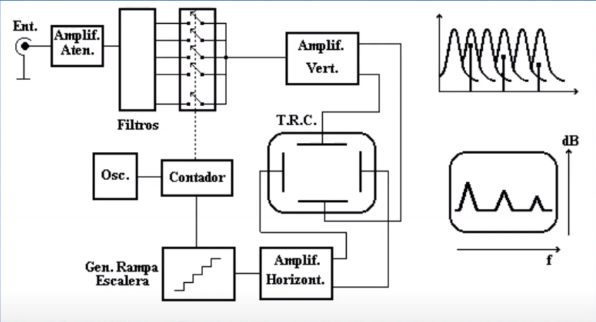
\includegraphics[width=\textwidth]{Imagenes/MarcoTeorico/EsqDeAnalizadorDeFourierBasico.png}}
          \caption{Esq. en bloques simplificador.}
          \label{fig:EsqAnalizadorDeFourierBasico}
        \end{subfigure}
        \caption{Analizar de fourier básico.}
        \label{fig:AnalizadorDeFourier}
      \end{figure}
           
    \subsubsection{Módulo matemático en Osciloscopios Digitales}

    Con la llegada de los osciloscopios digitales con módulo matemático, estos mismos 
    fueron reemplazando los analizadores de fourier convencionales.
    Dicho módulo posee un algoritmo de transformada rápida de fourier (FFT), donde 
    a partir de las muestras tomadas en el dominio del tiempo de una señal de entrada,
    se realiza la conversion de la señal con la FFT al dominio de la frecuencia.
    El esquema en bloques simplificado se puede observar en la Figura~\ref{fig:MathModuleEnOscil}.
        \begin{figure}[H]
            \centering
            \frame{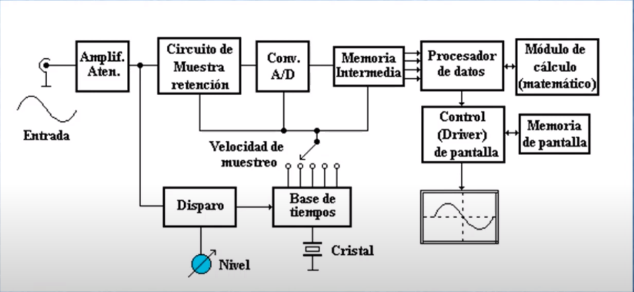
\includegraphics[width=\textwidth]{Imagenes/MarcoTeorico/MathModuleEnOscilDigital.png}}
            \caption{Módulo matemático en Osciloscopio Digital.}
            \label{fig:MathModuleEnOscil}
        \end{figure}
    
    En el modelo de Osciloscopio utilizado en el presente trabajo práctico (TP) 
    (\textit{Tektronix TDS 1001}), cuya presentación de pantalla se observa en la 
    Figura~\ref{fig:MathModoEnTek}.   
        \begin{figure}[H]
            \centering
            \frame{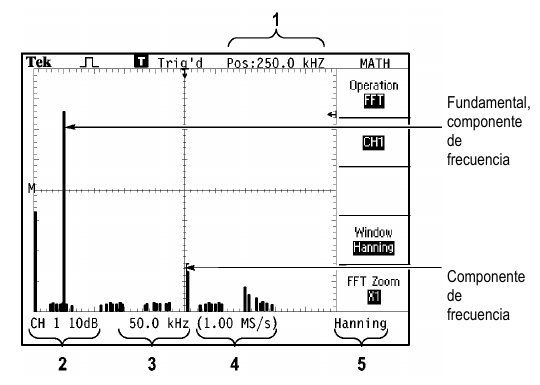
\includegraphics[width=\textwidth]{Imagenes/MarcoTeorico/PresentacionDePantallaFFT.png}}
            \caption{Modo Matemático en Osciloscopio,}
            \label{fig:MathModoEnTek}
        \end{figure}
    Donde se destaca los siguientes puntos 
    \begin{enumerate}
        \item Frecuencia de la linea central de la pantalla.
        \item Escala Vertical en dB/div donde (0 dB = 1 \(V_{RMS}\)).
        \item Escala horizontal en Frec/div.
        \item Velocidad de muestreo. 
        \item Tipo de ventana FFT. 
    \end{enumerate}    

     A continuación, se hace incapie en los tipos de ventanas que se utilizaran en el 
     presente TP como se observa en la Figura~\ref{fig:VentanasTipos} indicando sus 
     ventajas y desventajas.
        \begin{figure}[H]
            \centering
            \begin{subfigure}[H]{0.45\textwidth}
            \frame{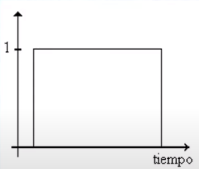
\includegraphics[width=\textwidth]{Imagenes/MarcoTeorico/VentanaRectangular.png}}
            \caption{Ventana Rectangular.}
            \label{fig:VentanaRec}
            \end{subfigure}
            \hfill 
            \begin{subfigure}[H]{0.45\textwidth}
            \frame{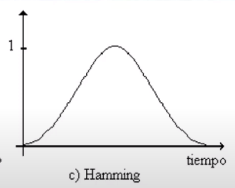
\includegraphics[width=\textwidth]{Imagenes/MarcoTeorico/VentanaHamming.png}} 
            \caption{Ventana Hamming.}
            \label{fig:VentanaHamming}
            \end{subfigure}
            \hfill 
            \begin{subfigure}[H]{0.45\textwidth}
            \frame{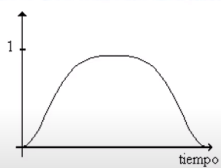
\includegraphics[width=\textwidth]{Imagenes/MarcoTeorico/VentanaFlattop.png}}
            \caption{Ventana flattop.}
            \label{fig:VentanaFlattop}
            \end{subfigure}

            \caption{Tipos de Ventan para FFT.}
            \label{fig:VentanasTipos}
        \end{figure}
    
    La \textbf{ventana rectangular}, Figura~\ref{fig:VentanaRec} posee como principal ventaja que son
    de gran utilidad para medir señales que poseen transitorios rápidos.
    como la ventana rectangular es una ventana de apertura y cierre abrupto, esto puede generar
    la aparición a flancos abruptos que no existen realmente en la señal, causando errores 
    en la lectura de la misma.
    
    La \textbf{ventana Hamming}, Figura~\ref{fig:VentanaHamming} se las concidera como una ventana de 
    apertura y cierre suave a diferencia de la rectangular. Esto permite eliminar el problema
    de los flancos abruptos facilitando las mediciones de amplitudes de las componentes 
    espectrales de una señal, pero como desventaja poseen poca exactitud para realizar 
    mediciones de frecuencias.
    
    Por último la \textbf{ventana flattop}, Figura~\ref{fig:VentanaFlattop} es una solución de compromiso
    entre las dos ventanas previamente mencionadas. 

    \subsubsection*{Uso de Cursores}
        
        Cabe destacar, que también se para realizar las mediciones en los diferentes ensayos
        se utiliza los \textbf{cursores} propios del osciloscopio. Con ellos se puede 
        realizar mediciones en amplitud (dB) o frecuencia tal como se observa en la
        Figura~\ref{fig:CursorTipos}.  
            \begin{figure}[H]
                \centering
                \begin{subfigure}[H]{0.45\textwidth}
                \frame{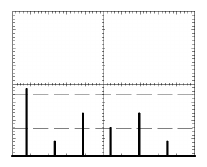
\includegraphics[width=\textwidth]{Imagenes/MarcoTeorico/CursoresEnMagnitud.png}}
                \caption{Cursores en Magnitud.}
                \label{fig:CursorMag}
                \end{subfigure}
                \hfill 
                \begin{subfigure}[H]{0.45\textwidth}
                \frame{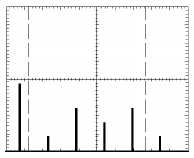
\includegraphics[width=\textwidth]{Imagenes/MarcoTeorico/CursoresEnFrecuencia.png}}
                \caption{Cursores en Frecuencia.}
                \label{fig:CursorFrec}
                \end{subfigure}
                \caption{Tipos de cursores del Osciloscopio Digital.}
                \label{fig:CursorTipos}
            \end{figure}

        Se debe tener presente que cuandos e realiza mediciones en magnitud en frecuencia con 
        el osciloscopio, dicha magnitud dada en decibleles esta referenciada a valor de RMS
        y no de amplitud pico de la señal.
                
    

    









    \pagebreak
  \section{Actividad Práctica}
    Se propone como actividad realizar el análisis de distintas señales en la frecuencia con el uso del
    módulo matemático de un osciloscopio digital, mediante la FFT. Con este objetivo, los instrumentos
    e insumos necesarios son:

    \begin{itemize}
      \item Osciloscopio digital Tektronix TDS 1001
      \item 2 generadores de señal Goldstar FG-8002
      \item Multímetro RMS MARCA Y MODELOOOOOOO
      \item Circuito modulador de amplitud con diodo y circuito sintonizado
      \item Potenciómetro de $1~k\Omega$
      \item Amplificador transistorizado de dos etapas
    \end{itemize}

    \input{Secciones/Subsecciones/1AnalisisDeUnaSeñalCuadrada.tex}
      \subsection{Análisis de un tren de pulsos}

    Se analiza a continuación una señal con forma de onda de tren de pulsos rectangulares, en el dominio 
    de la frecuencia.
    Se sabe que la relación de período en el dominio del tiempo y ancho de banda en el dominio de la frecuencia, 
    es inversamente proporcional. Es por ello, que se utiliza una señal de pulsos rectangulares, para poder visualizar 
    dicha relación.

    Se configura el generador de la siguiente manera: período de $\mathbf{1~ms}$, ancho de pulso de 
    $\mathbf{250~} \boldsymbol{\mu} \mathbf{s}$, y se gira media vuelta la perilla de control de amplitud.
    El ajuste del generador se observa en el osciloscopio en la Figura~\ref{fig:Exp2SeñalPulso}.

      \begin{figure}[H]
        \centering
        \begin{subfigure}[H]{0.48\textwidth}
          \frame{\includegraphics[width=\textwidth]{Imagenes/ActividadPractica/2AnalisisDeUnTrenDePulsos/Exp2_PeriodoDeLaSeñalDeEntrada.jpeg}}
          \caption{Señal pulsante de período de $1~ms$.}
        \end{subfigure}
        \hfill
        \begin{subfigure}[H]{0.48\textwidth}
          \frame{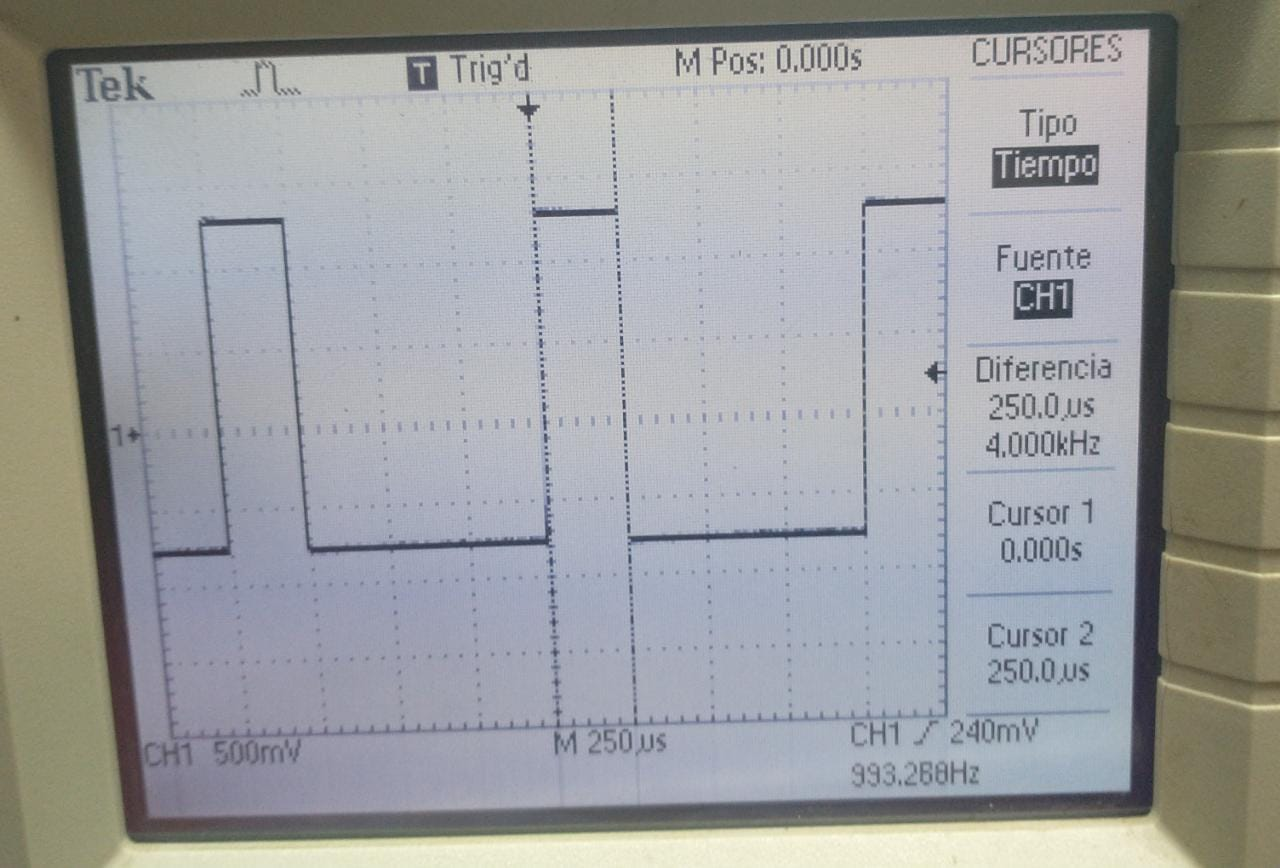
\includegraphics[width=\textwidth]{Imagenes/ActividadPractica/2AnalisisDeUnTrenDePulsos/Exp2_AnchoDelPulsoDeEntrada.jpeg}}
          \caption{Ancho del pulso de $250~\mu s$.}
        \end{subfigure}

        \caption{Tren de pulsos.}
        \label{fig:Exp2SeñalPulso}
      \end{figure}

    Ahora, se cambia al modo matemático a través del botón \textbf{MATH MENU}, y se configura con: \textbf{FFT}, 
    \textbf{CH1}, \textbf{Rectangular}, \textbf{Zoom X1} y modo adquisición \textbf{Promedio} en 64 muestras. 
    Dicha configuración se enseña en la Figura~\ref{fig:Exp2SeñalPulsanteEspectro}.

      \begin{figure}[H]
        \centering
          \frame{\includegraphics[width=0.48\textwidth]{Imagenes/ActividadPractica/2AnalisisDeUnTrenDePulsos/Exp2_EspectroDeLaSeñalPulsante.jpeg}}
          \caption{Análisis en frecuencia de la señal de entrada.}
          \label{fig:Exp2SeñalPulsanteEspectro}
      \end{figure}

      Luego, se observa cómo varía el espectro entre los 3 tipos de ventana: \textbf{Hanning}, \textbf{Rectangular}, 
      y \textbf{Flattop}, lo cual se ve en la Figura~\ref{fig:Exp2SeñalPulsanteVentanasEspectro}.

      \begin{figure}[H]
        \centering
        \begin{subfigure}[H]{0.48\textwidth}
          \frame{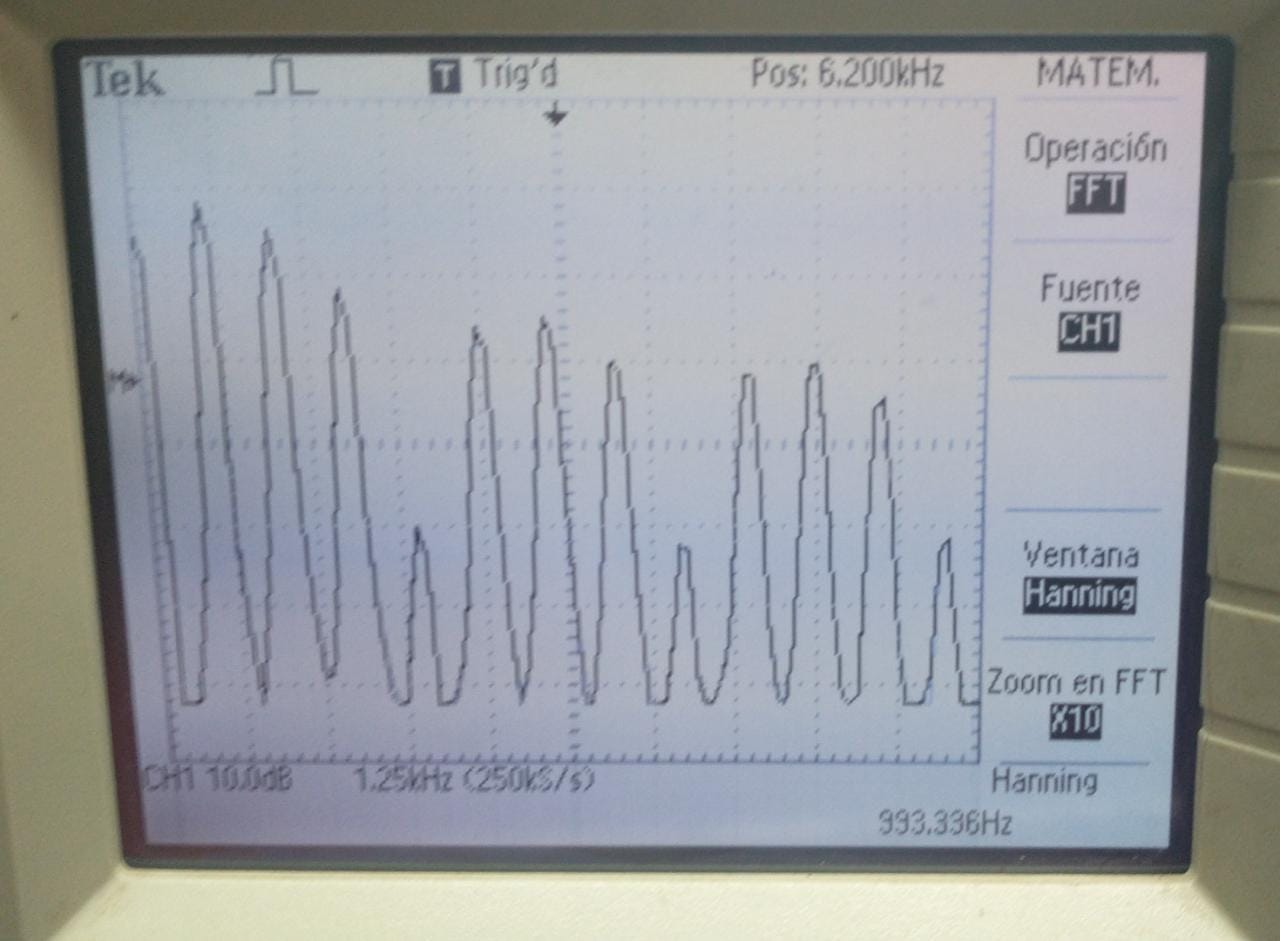
\includegraphics[width=\textwidth]{Imagenes/ActividadPractica/2AnalisisDeUnTrenDePulsos/Exp2_EspectroEnVentanaHannin.jpeg}}
          \caption{Ventana Hanning.}
        \end{subfigure}
        \hfill
        \begin{subfigure}[H]{0.48\textwidth}
          \frame{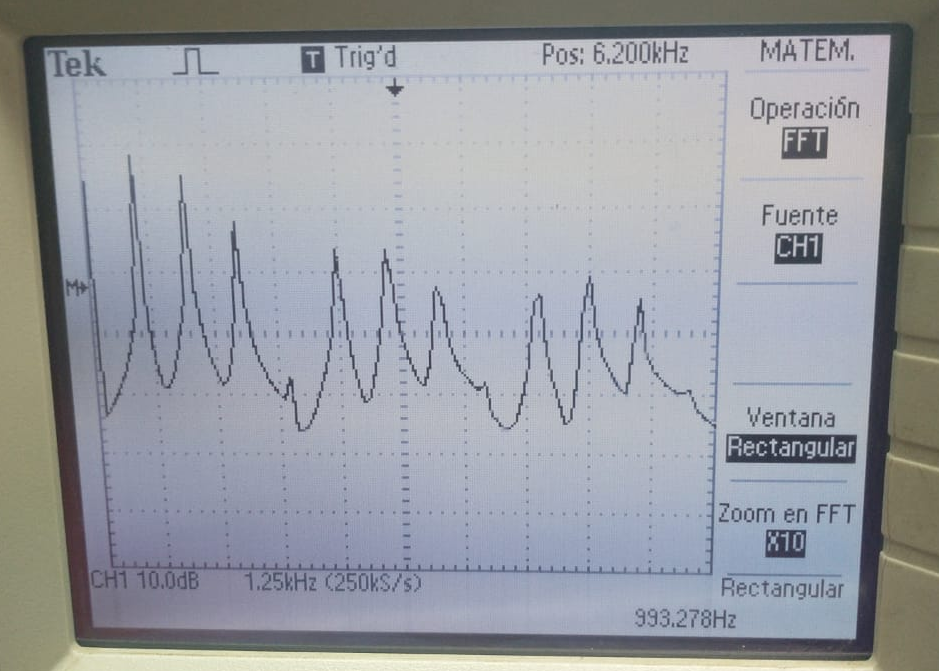
\includegraphics[width=\textwidth]{Imagenes/ActividadPractica/2AnalisisDeUnTrenDePulsos/Exp2_EspectroEnVentanaRectangular.png}}
          \caption{Ventana Rectangular.}
        \end{subfigure}
        \begin{subfigure}[H]{0.48\textwidth}
          \frame{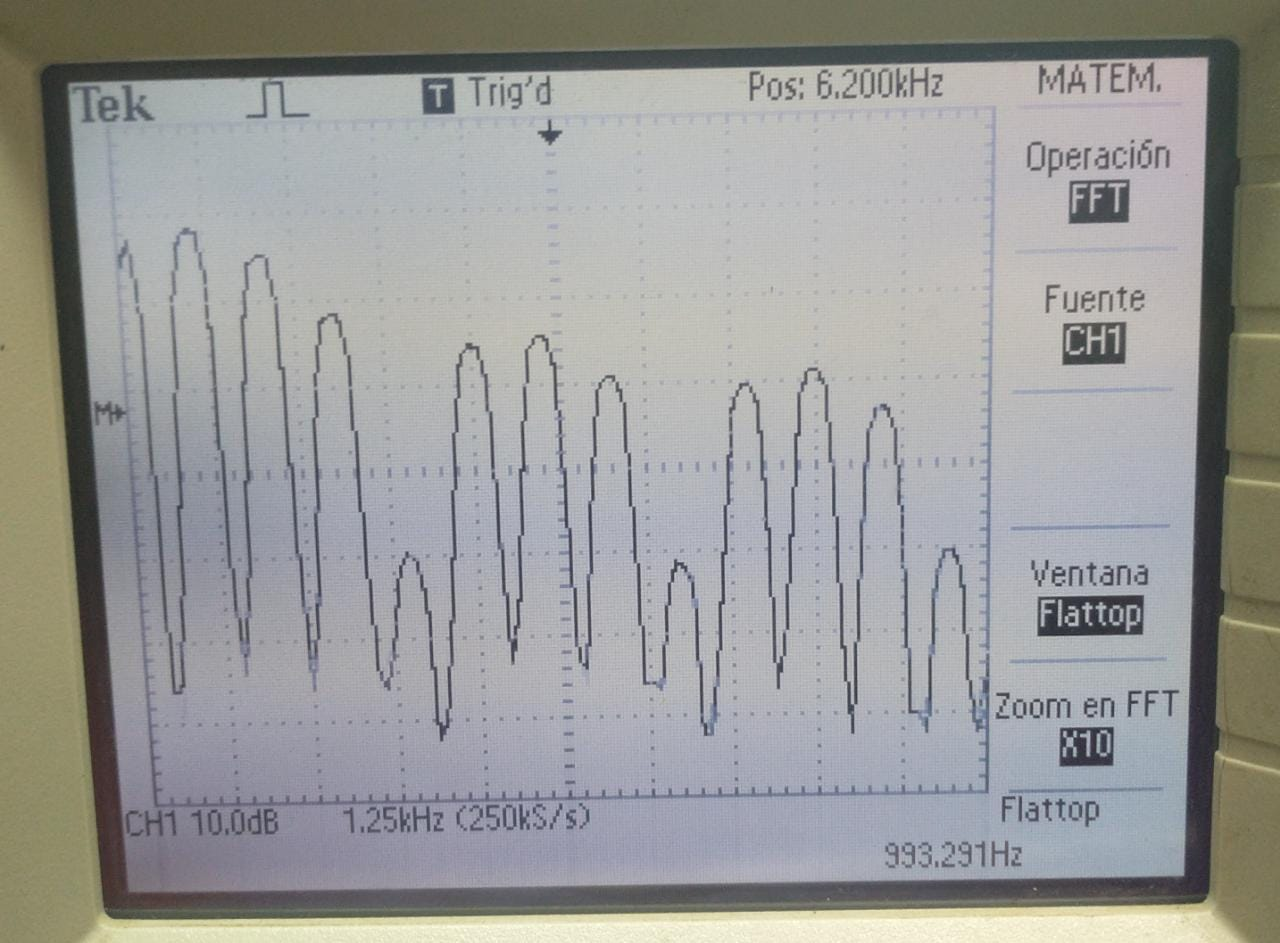
\includegraphics[width=\textwidth]{Imagenes/ActividadPractica/2AnalisisDeUnTrenDePulsos/Exp2_EspectroEnVentanaFlattop.jpeg}}
          \caption{Ventana Flattop.}
        \end{subfigure}

        \caption{Análisis en frecuencia con las distintas ventanas.}
        \label{fig:Exp2SeñalPulsanteVentanasEspectro}
      \end{figure}

      A continuación, se selecciona ventana \textbf{Rectangular}, se coloca el menú de cursores, y se selecciona 
      \textbf{frecuencia} en fuente 
      \textbf{Matemático}. Se coloca el \textbf{Cursor 1}, en $0~Hz$ y con el \textbf{Cursor 2} se 
      procede a medir las frecuencias de cada pico, como muestra la 
      Figura~\ref{fig:Exp2SeñalPulsanteArmonicosEspectro}.

       \begin{figure}[H]
        \centering
        \begin{subfigure}[H]{0.48\textwidth}
          \frame{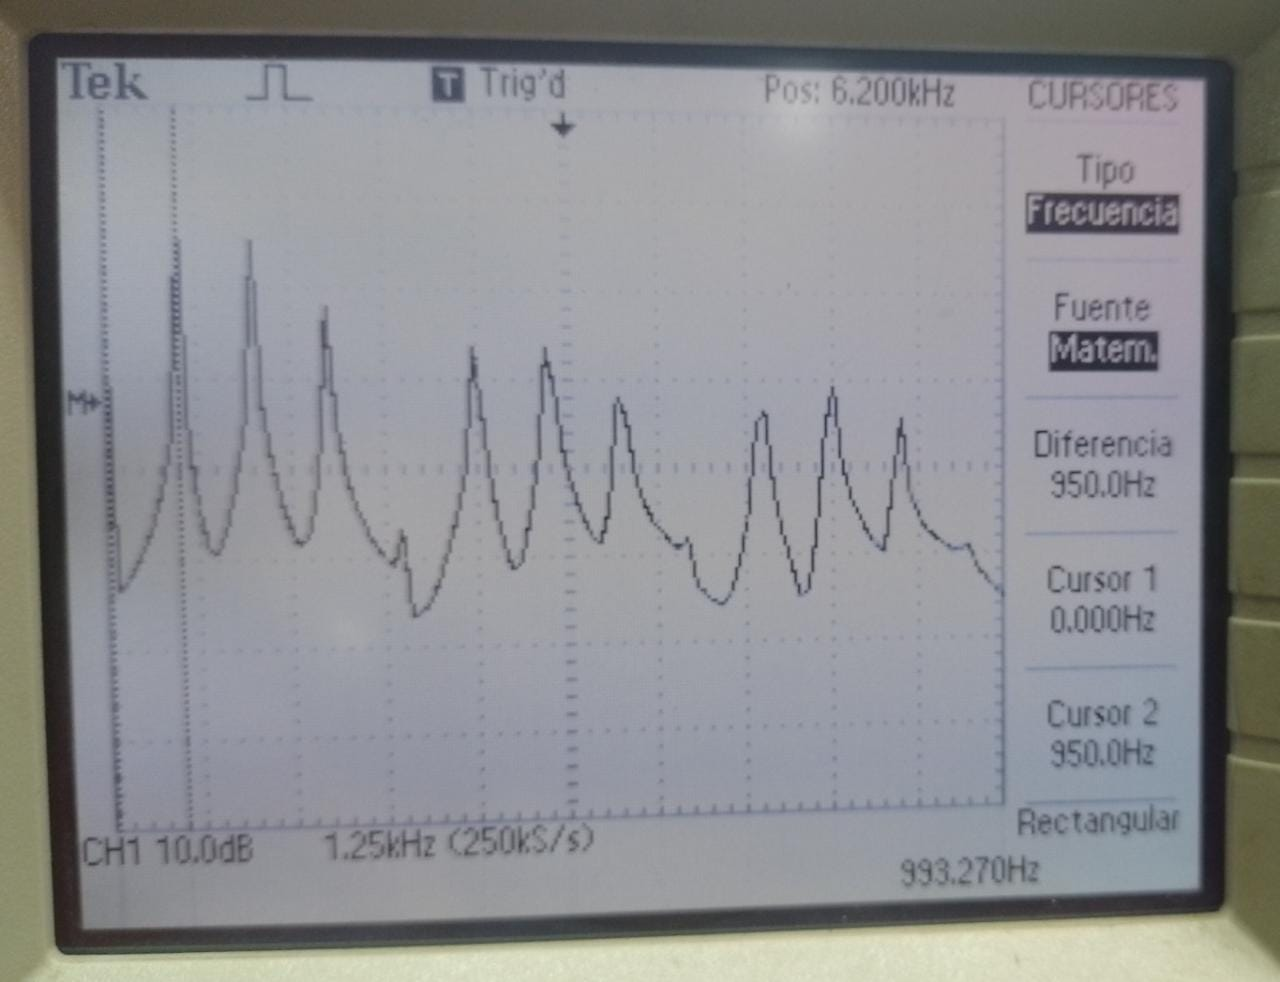
\includegraphics[width=\textwidth]{Imagenes/ActividadPractica/2AnalisisDeUnTrenDePulsos/Exp2_FrecArmonico1.jpeg}}
          \caption{Frecuencia de la fundamental en ventana Rectangular, $f_{1}=950~Hz$.}
        \end{subfigure}
        \hfill
        \begin{subfigure}[H]{0.48\textwidth}
          \frame{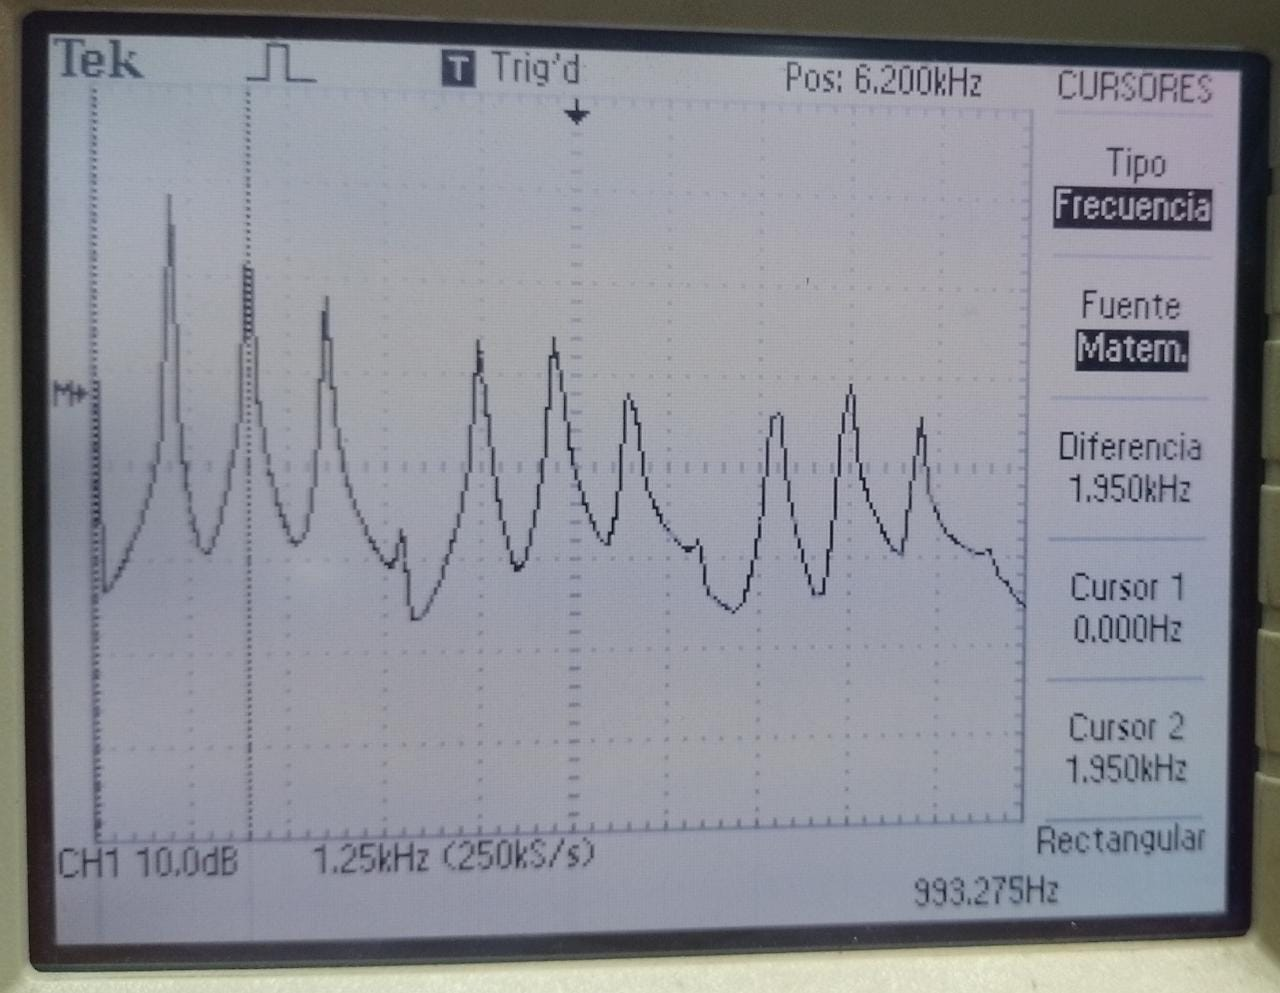
\includegraphics[width=\textwidth]{Imagenes/ActividadPractica/2AnalisisDeUnTrenDePulsos/Exp2_FrecArmonico2.jpeg}}
          \caption{Frecuencia de la segunda armónica en ventana Rectangular, $f_{2}=1950~Hz$.}
        \end{subfigure}
        \begin{subfigure}[H]{0.48\textwidth}
          \frame{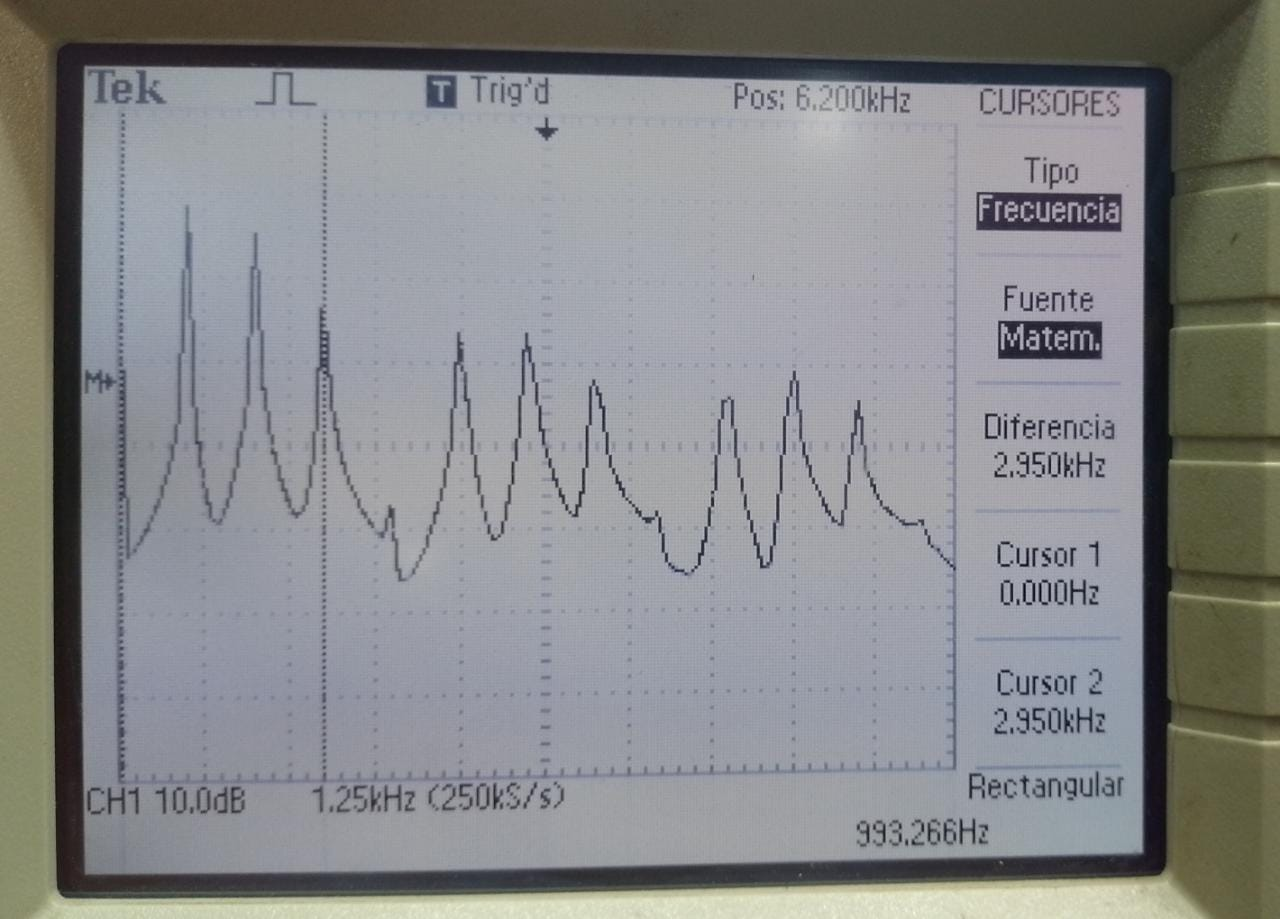
\includegraphics[width=\textwidth]{Imagenes/ActividadPractica/2AnalisisDeUnTrenDePulsos/Exp2_FrecArmonico3.jpeg}}
          \caption{Frecuencia de la tercera armónica en ventana Rectangular, $f_{3}=2950~Hz$.}
        \end{subfigure}
       \hfill
        \begin{subfigure}[H]{0.48\textwidth}
          \frame{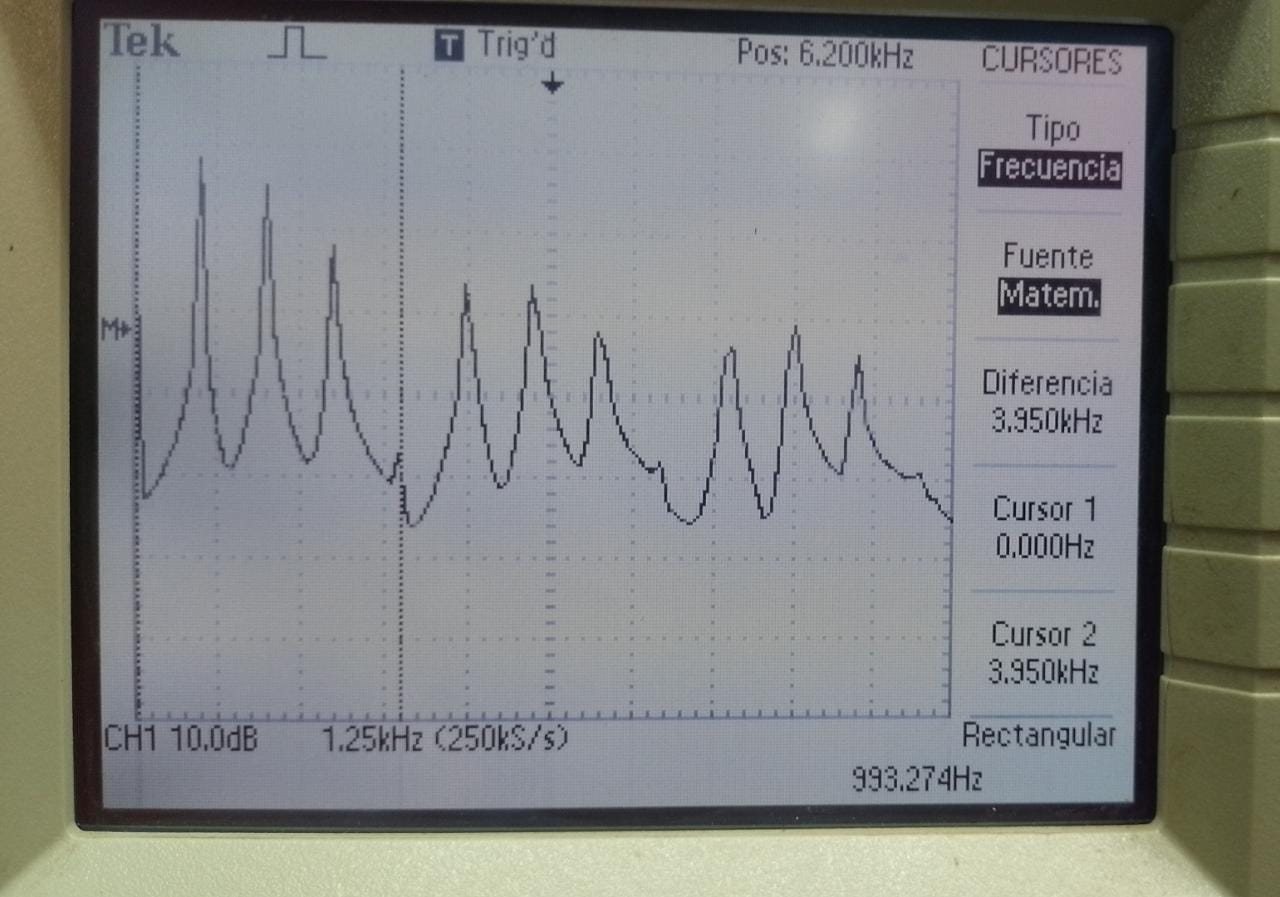
\includegraphics[width=\textwidth]{Imagenes/ActividadPractica/2AnalisisDeUnTrenDePulsos/Exp2_FrecArmonico4.jpeg}}
          \caption{Frecuencia de la cuarta armónica en ventana Rectangular, $f_{4}=3950~Hz$.}
        \end{subfigure}
        \begin{subfigure}[H]{0.48\textwidth}
          \frame{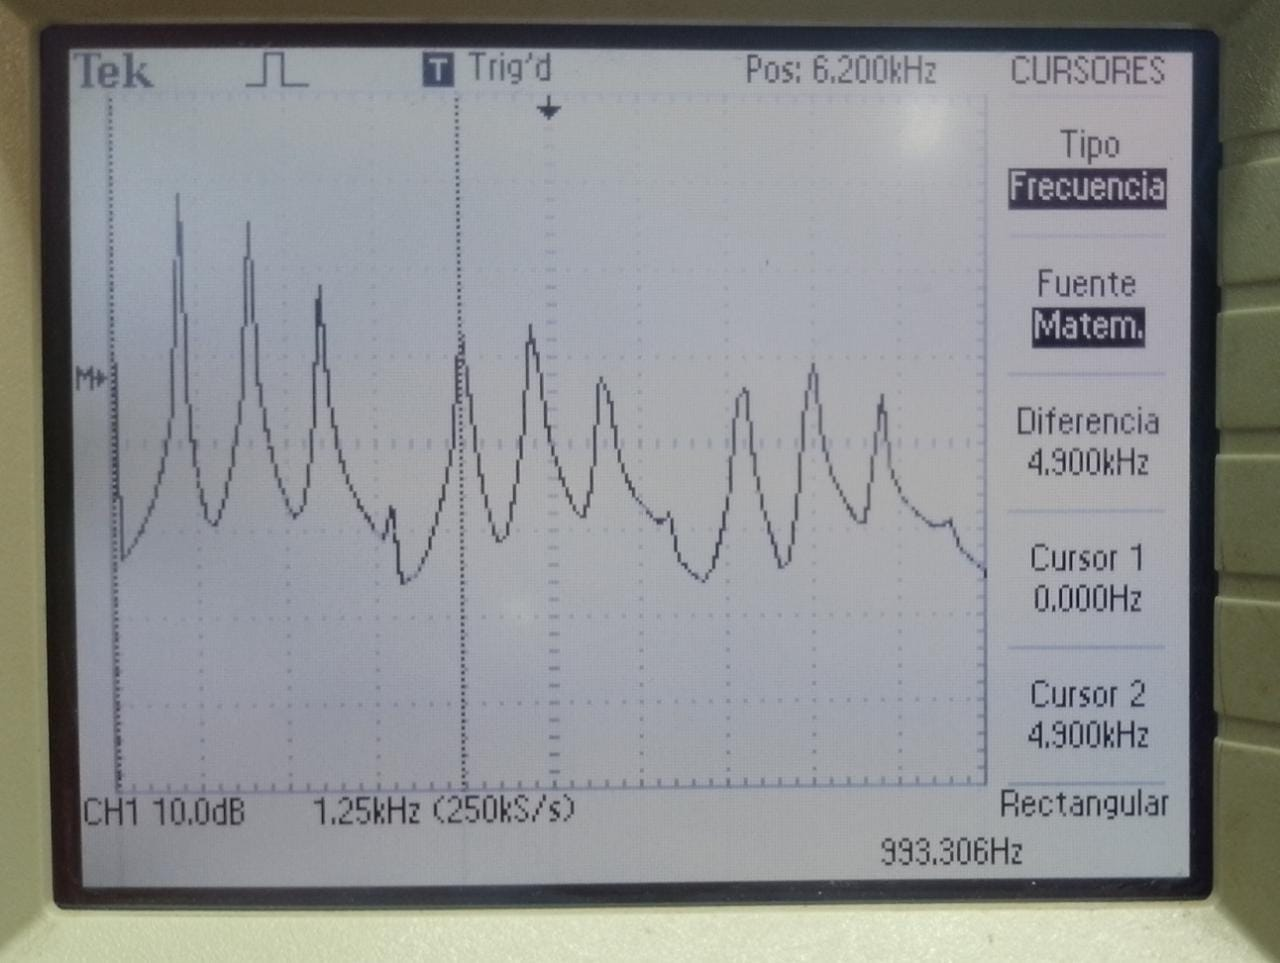
\includegraphics[width=\textwidth]{Imagenes/ActividadPractica/2AnalisisDeUnTrenDePulsos/Exp2_FrecArmonico5.jpeg}}
          \caption{Frecuencia de la quinta armónica en ventana Rectangular, $f_{5}=4900~Hz$.}
        \end{subfigure}

        \caption{Medición de frecuencia de picos de la señal pulsante en ventana Rectangular.}
        \label{fig:Exp2SeñalPulsanteArmonicosEspectro}
      \end{figure}     

      Se confecciona una tabla con las \textbf{diferencias de frecuencia} entre picos, en 
      base a las mediciones realizadas. Los valores se encuentran en la 
      Tabla~\ref{tab:Exp2MedicionesHanning}.

      \begin{table}[H]
      \centering
        \begin{tabular}{cccccc} \hline \hline
          \textbf{Cursor 2}               &  $\mathbf{1erArm.}$       & $\mathbf{2daArm.}$        & $\mathbf{3raArm.}$  &   $\mathbf{4taArm.}$ &   $\mathbf{5taArm.}$ \\ \hline
          $\mathbf{\Delta f_{n}~[Hz]}$     &   $950$                   &    $1000$                  &   $1000$             & $1000$                & $950$                \\ \hline \hline
         \end{tabular}
          \caption{Valores de frecuencia medidos en ventana Hanning.}
          \label{tab:Exp2MedicionesHanning}
      \end{table}

      Se calcula el promedio de las frecuencias como sigue
      \begin{align*}
        \Delta f_{n_{prom}}=\dfrac{\sum{\Delta_{fn}}}{n} \hspace{20pt} \therefore \hspace{20pt} \boxed{\Delta_{fn_{prom}}=980~[Hz]}~,
      \end{align*}
      y el período de la onda de pulsos es 
      \begin{align*}
        Periodo~\left( T \right)=\dfrac{1}{\Delta f_{n_{prom}}} \hspace{20pt} \therefore \hspace{20pt} \boxed{Periodo~\left( T \right)=1,02~[ms]}~.
      \end{align*}

        Se repite el experimento utilizando la ventana \textbf{Flattop}, pero ésta vez se miden los 
        \textbf{valles} que presenta el espectro, que se visualiza en la 
        Figura~\ref{fig:Exp2SeñalPulsanteVallesEspectro}.

       \begin{figure}[H]
        \centering
        \begin{subfigure}[H]{0.48\textwidth}
          \frame{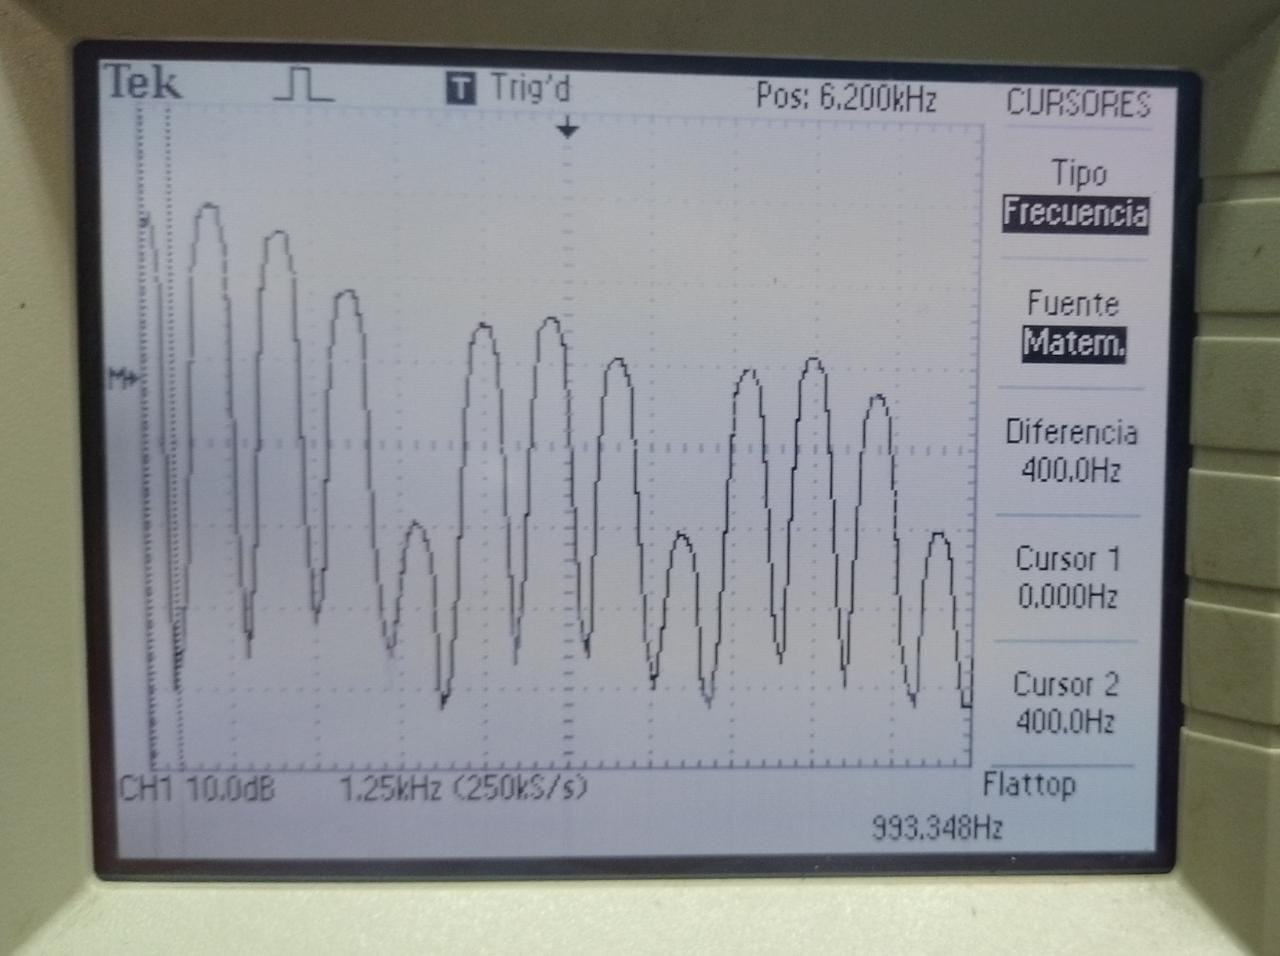
\includegraphics[width=\textwidth]{Imagenes/ActividadPractica/2AnalisisDeUnTrenDePulsos/Exp2_FrecValle1Flattop.jpeg}}
          \caption{Frecuencia del primer valle en ventana Flattop, $f_{a}=400~Hz$.}
        \end{subfigure}
        \hfill
        \begin{subfigure}[H]{0.48\textwidth}
          \frame{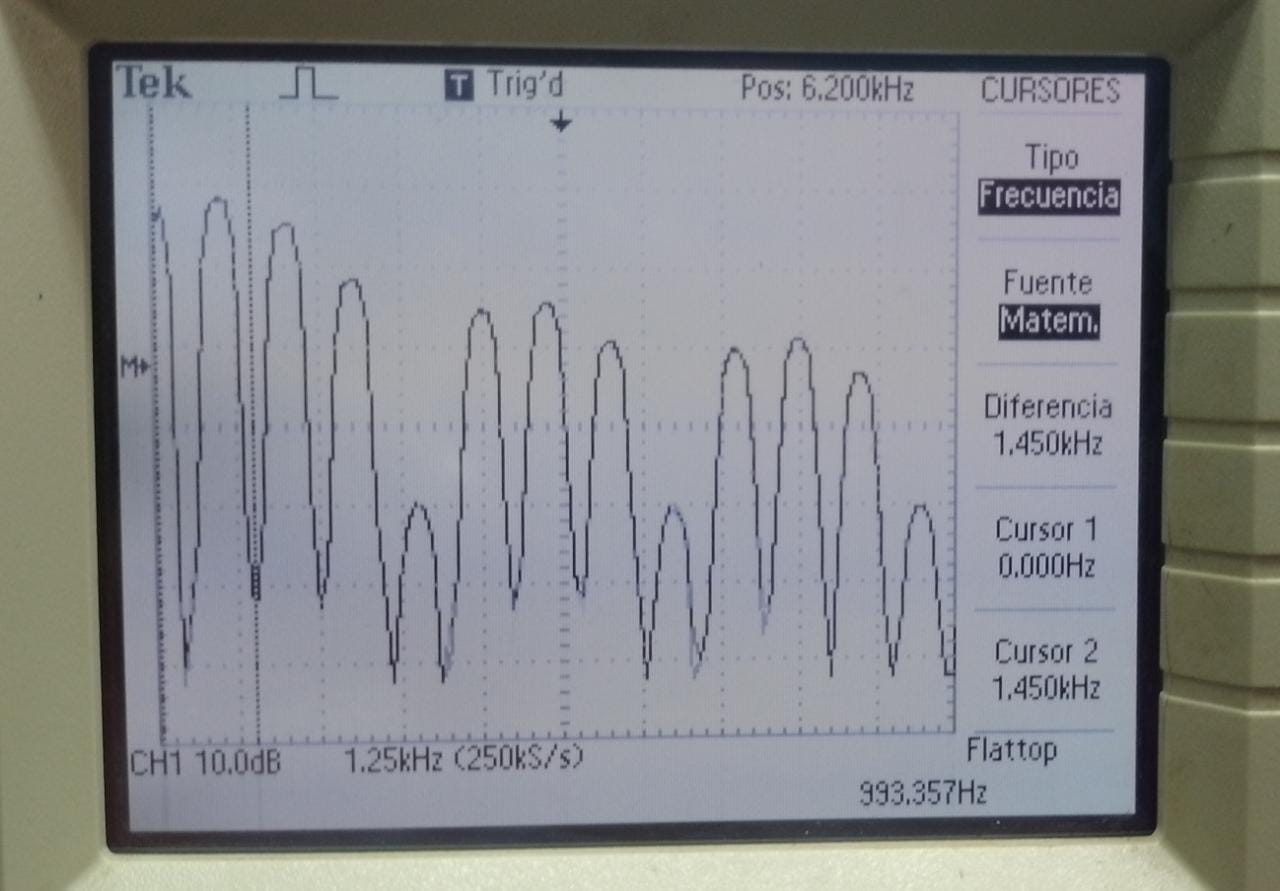
\includegraphics[width=\textwidth]{Imagenes/ActividadPractica/2AnalisisDeUnTrenDePulsos/Exp2_FrecValle2Flattop.jpeg}}
          \caption{Frecuencia del segundo valle en ventana Flattop, $f_{b}=1450~Hz$.}
        \end{subfigure}
        \hfill
        \begin{subfigure}[H]{0.48\textwidth}
          \frame{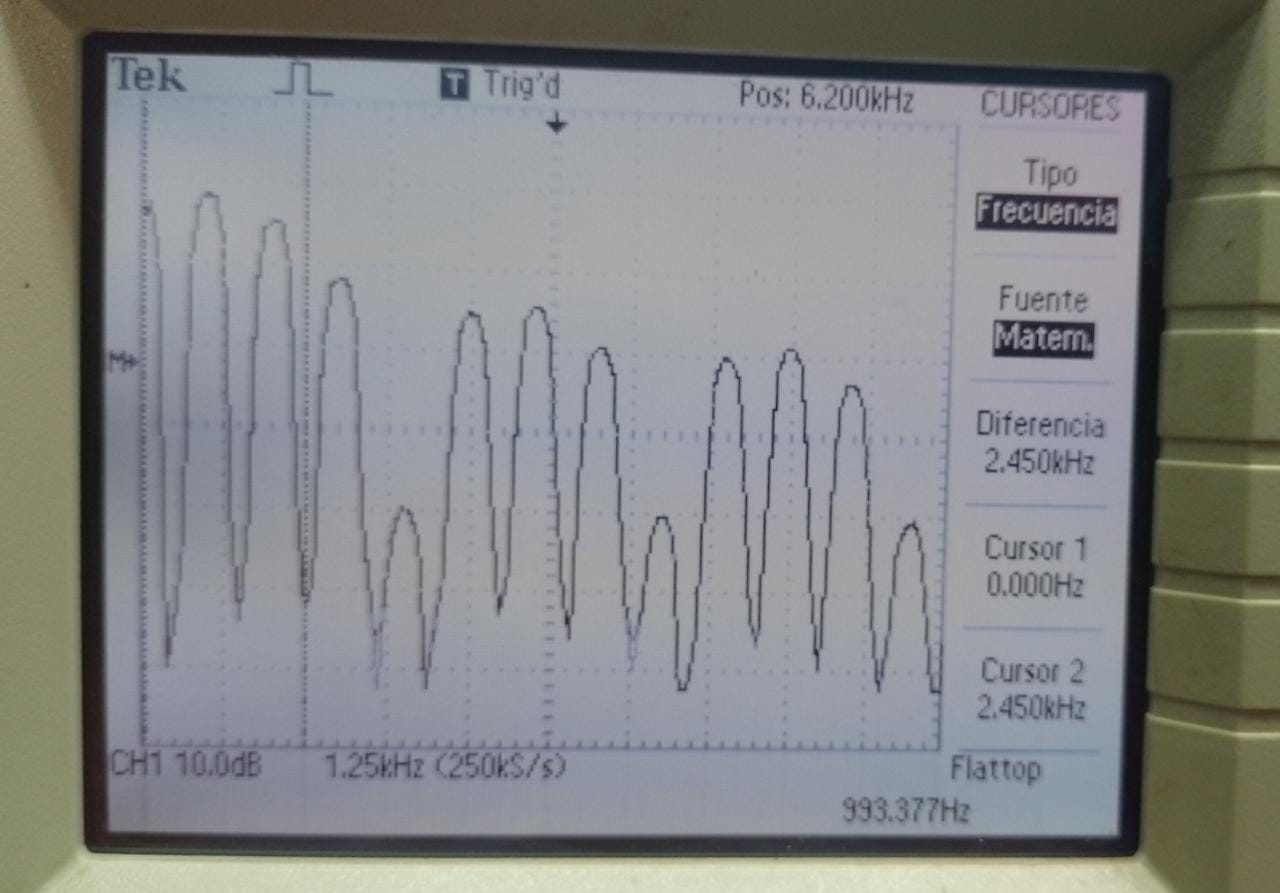
\includegraphics[width=\textwidth]{Imagenes/ActividadPractica/2AnalisisDeUnTrenDePulsos/Exp2_FrecValle3Flattop.jpeg}}
          \caption{Frecuencia del tercer valle en ventana Flattop, $f_{c}=2450~Hz$.}
        \end{subfigure}

        \caption{Medición de frecuencia de valles de la señal pulsante en ventana Flattop.}
        \label{fig:Exp2SeñalPulsanteVallesEspectro}
      \end{figure}     

      Se confecciona una tabla con los valores obtenidos, los mismos se encuentran en la 
      Tabla~\ref{tab:Exp2MedicionesFlattop}, y se calculan nuevamente el $\Delta f_{n_{prom}}$
      y el período. 

      \begin{table}[H]
      \centering
        \begin{tabular}{ccc} \hline \hline
          $\mathbf{\Delta_{fmin1}}$               &  $\mathbf{\Delta_{fmin2}}$       & $\mathbf{\Delta_{fmin3}}$ \\ \hline
                    $400~Hz$                        &    $1050~Hz$                    &   $1000~Hz$  \\ \hline \hline
         \end{tabular}
          \caption{Valores de frecuencia medidos en ventana Flattop.}
          \label{tab:Exp2MedicionesFlattop}
      \end{table}  

      \begin{align*}
        \Delta_{fn_{prom}}=\dfrac{\sum{\Delta_{fn}}}{n} \hspace{20pt} \therefore \hspace{20pt} \boxed{\Delta_{fn_{prom}}=816,67~[Hz]}
      \end{align*}        

      \begin{align*}
        Periodo~\left( T \right)=\dfrac{1}{\Delta_{fn_{prom}}} \hspace{20pt} \therefore \hspace{20pt} \boxed{Periodo~\left( T \right)=1,224~[ms]}
      \end{align*}

      Finalmente, se mide la amplitud de la frecuencia correspondiente a $0~Hz$, y se mide 
      también con multímetro el nivel de continua de la señal, posteriormente se comparan 
      los resultados.

       \begin{figure}[H]
        \centering
        \begin{subfigure}[H]{0.48\textwidth}
          \frame{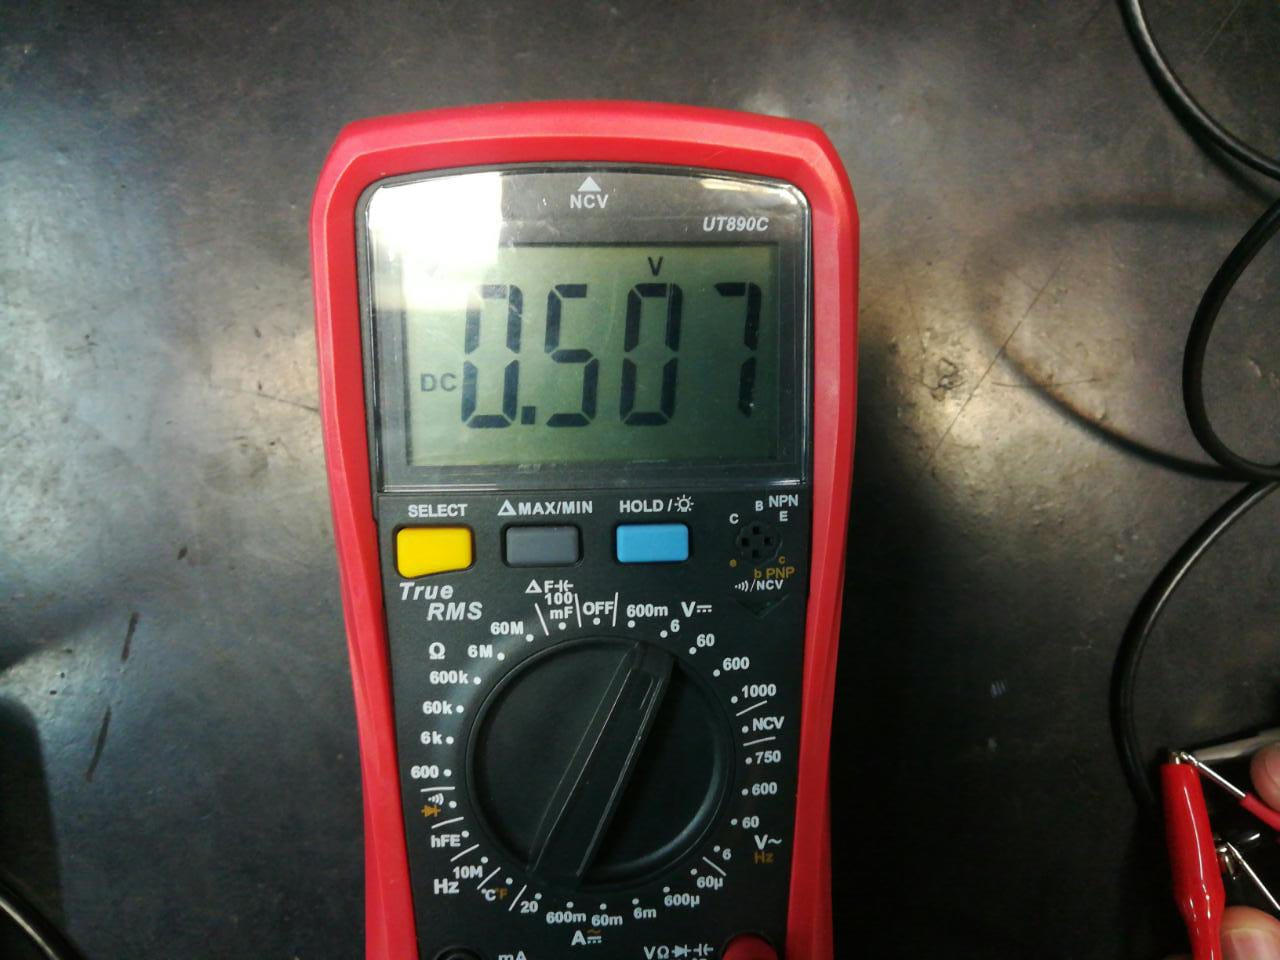
\includegraphics[width=\textwidth]{Imagenes/ActividadPractica/2AnalisisDeUnTrenDePulsos/MedicionCCOscilo.jpeg}}
          \caption{Medición de continua con osciloscopio, $CC_{osc}=1~V$.}
        \end{subfigure}
        \hfill
        \begin{subfigure}[H]{0.48\textwidth}
          \frame{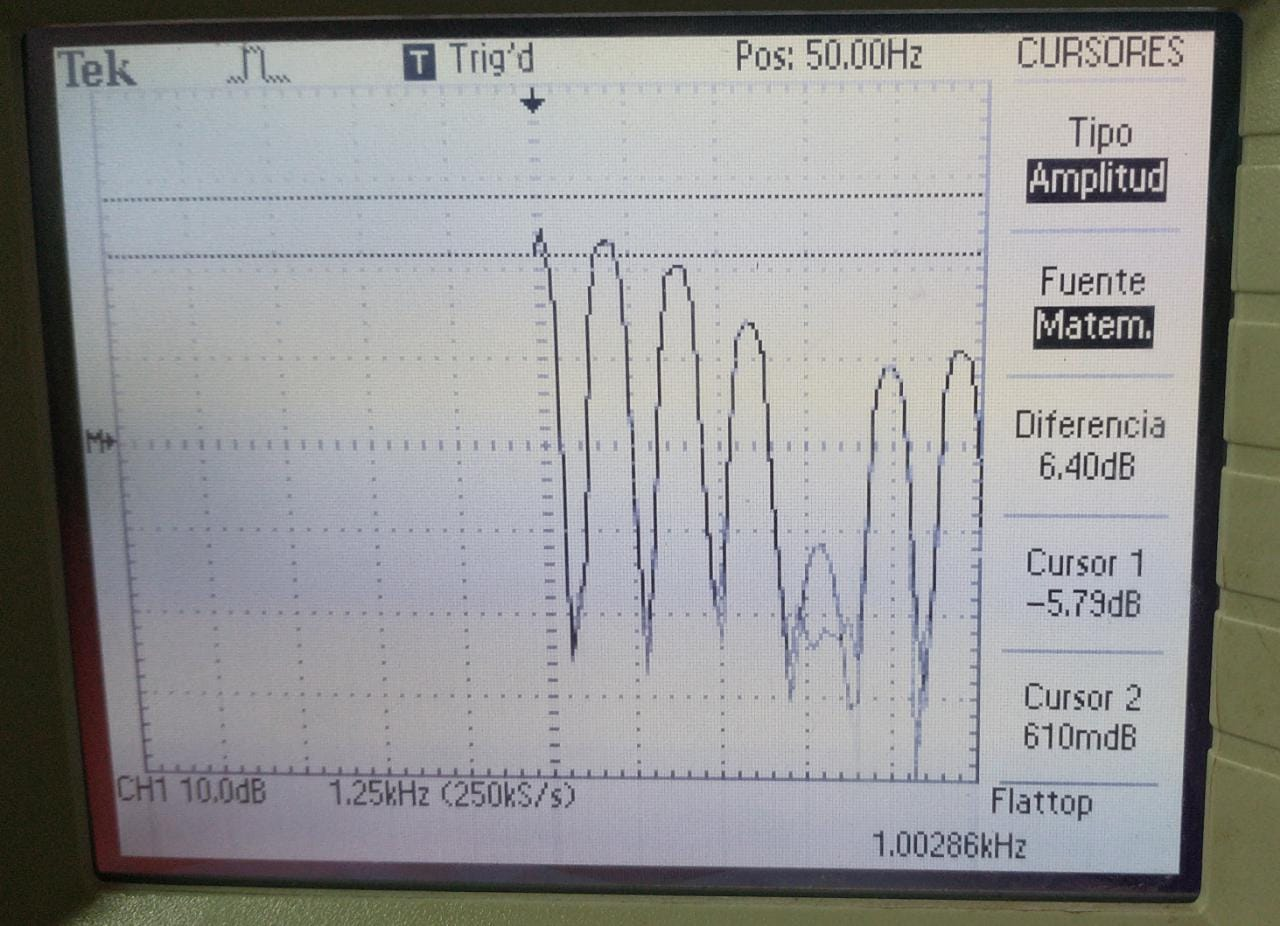
\includegraphics[width=\textwidth]{Imagenes/ActividadPractica/2AnalisisDeUnTrenDePulsos/MedicionCCMultiM.jpeg}}
          \caption{Medición de continua con multímetro, $CC_{Mult}=1~V$.}
        \end{subfigure}

        \caption{Medición del nivel de continua de la señal pulsante.}
        \label{fig:Exp2SeñalPulsanteContinua}
      \end{figure}        

      La medición realizada con el osciloscopio da como resultado $V_{rms}=0,513~V$, lo cual coincide con la medición realizada
      con el multímetro.


      \subsection{Obervación de frecuencias producto del aliasing}

    \input{Secciones/Subsecciones/4AnalisisDeUnaSeñalDeAM.tex}
      \subsection{Observación de los productos de IMD de tercer orden}
    En la experiencia anterior se hace uso de un diodo para poder generar la modulación de
    amplitud. El circuito en cuestión se puede ver en la Figura~\ref{fig:ModuladorAM} de
    la Sección~\ref{sec:Exp4_AM}.

    Este dispositivo tiene un comportamiento alineal, el cual se puede modelar
    de la siguiente  forma

    \vspace{-10pt}
    \begin{equation*}
      v_{AM} = k_a(v_{G1}+v_{G2}) + k_b(v_{G1}+v_{G2})^2 + k_c(v_{G1}+v_{G2})^3 + \cdots
    \end{equation*}
    donde es de especial interés la región cuadrática de este dispositivo, ya que,
    debido a este, se obtiene la modulación de amplitud buscada. Si se 
    desarrolla el término correspondiente (el cuadrático), se logra justificar lo
    mencionado
    
    \vspace{-10pt}
    \begin{equation*}
      v_{AM} = \cdots + k_b(v_{G1}^2 + 2\cdot{v_{G1}v_{G2}} + v_{G2}^2) + \cdots ~.
    \end{equation*}

    Por el contrario, las \textbf{alinealidades de orden superior} dan como resultado \textbf{productos
    de intermodulación} (\textbf{IMD}), los cuales son efectos no deseados. La alinealidad más
    importante suele ser la IMD de tercer orden, por lo cual, ahora se procede a determinar el
    \textbf{rechazo de IMD de tercer orden} del circuito modulador utilizado.

    Para ello, se setean ambos generadores \textbf{G1} y \textbf{G2} a una frecuencia de 
    \textbf{f=50~kHz}, y a \textbf{igual amplitud}. Luego, se observan las señales de salida del circuito 
    dejando un solo generador encendido. Los resultados se encuentran en las Figuras~\ref{fig:SalidaCircuitConG1Encendido}
    y \ref{fig:SalidaCircuitConG2Encendido}.


    \begin{figure}[H]
      \centering
      \begin{subfigure}[H]{0.48\textwidth}
        \frame{\includegraphics[width=\textwidth]{Imagenes/ActividadPractica/5ProductosDeIMPde3erOrden/Exp5_SeñalSalidaConG1Autoset_Tiempo.jpeg}}
        \caption{En tiempo.}
      \end{subfigure}
      \hfill 
      \begin{subfigure}[H]{0.48\textwidth}
        \frame{\includegraphics[width=\textwidth]{Imagenes/ActividadPractica/5ProductosDeIMPde3erOrden/Exp5_SeñalSalidaConG1_Frecuencia.jpeg}}
        \caption{En frecuencia.}
      \end{subfigure}

      \caption{Salida del circuito con el generador G1 encendido.}
      \label{fig:SalidaCircuitConG1Encendido}
    \end{figure}


    \begin{figure}[H]
      \centering
      \begin{subfigure}[H]{0.48\textwidth}
        \frame{
\includegraphics[width=\textwidth]{Imagenes/logo-utn.png}}
        \caption{En tiempo.}
      \end{subfigure}
      \hfill 
      \begin{subfigure}[H]{0.48\textwidth}
        \frame{\includegraphics[width=\textwidth]{Imagenes/ActividadPractica/5ProductosDeIMPde3erOrden/Exp5_SeñalSalidaConG2_Frecuencia.jpeg}}
        \caption{En frecuencia.}
      \end{subfigure}

      \caption{Salida del circuito con el generador G2 encendido.}
      \label{fig:SalidaCircuitConG2Encendido}
    \end{figure}

    A continuación, se encienden ambos generadores y se ajusta el tiempo de muestreo y se habilita el \textbf{Zoom x10}
    para obtener una mejor visualización. Luego, se procede a separar ambas señales un ancho de $\mathbf{\triangle f=  2~kHz}$,
    quedando una de ellas en $\mathbf{f_1=49~kHz}$ y la otra en $\mathbf{f_2=51~kHz}$. En la
    Figura~\ref{fig:SalidaConAmbosGeneradores} se puede ver lo explicado en este párrafo.

    \begin{figure}[H]
      \centering
      \begin{subfigure}[H]{0.48\textwidth}
        \frame{\includegraphics[width=\textwidth]{Imagenes/ActividadPractica/5ProductosDeIMPde3erOrden/Exp5_SeñalSalidaConLosDosGeneradores_Frec.jpeg}}
        \caption{Ambas a la misma frecuencia.}
      \end{subfigure}
      \hfill 
      \begin{subfigure}[H]{0.48\textwidth}
        \frame{\includegraphics[width=\textwidth]{Imagenes/ActividadPractica/5ProductosDeIMPde3erOrden/Exp5_SeparacionDeSeñalesDe2KHz.jpeg}}
        \caption{Con separación de $2~kHz$.}
      \end{subfigure}

      \caption{Espectro de la señal de salida con ambas señales inyectadas al circuito.}
      \label{fig:SalidaConAmbosGeneradores}
    \end{figure}

    Las componentes de $\mathbf{47~kHz}\  (2f_1 - f2)$ y $\mathbf{53~kHz}\  (2f_2 - f1)$ son los productos de IMD de tercer orden. Para obtenerlos
    se realiza la diferencia en amplitud entre estas y \textbf{f\textsubscript{1}} y \textbf{f\textsubscript{2}} respectivamente. Dichas mediciones,
    realizadas con la ventana \textbf{Hanning}, se pueden ver en la Figura~\ref{fig:MedicionIMD}.

    \begin{figure}[H]
      \centering
      \begin{subfigure}[H]{0.48\textwidth}
        \frame{\includegraphics[width=\textwidth]{Imagenes/ActividadPractica/5ProductosDeIMPde3erOrden/Exp5_IDM3erOrdenConSeñal49kHz.jpeg}}
        \caption{Para $f_1=49~kHz$.}
      \end{subfigure}
      \hfill 
      \begin{subfigure}[H]{0.48\textwidth}
        \frame{\includegraphics[width=\textwidth]{Imagenes/ActividadPractica/5ProductosDeIMPde3erOrden/Exp5_IDM3erOrdenConSeñal51kHz.jpeg}}
        \caption{Para $f_2=51~kHz$.}
      \end{subfigure}

      \caption{Medición de diferencia de amplitudes.}
      \label{fig:MedicionIMD}
    \end{figure}

    Los valores obtenidos de esta experiencia se encuentran tabulados en la Tabla~\ref{tab:DatosDeMedicionDeIMD}.

    \begin{table}[H]
      \centering
    \begin{tabular}{ccccc} \hline \hline
      $\mathbf{f_{1}}$    &   $\mathbf{f_{2}}$  &  $\mathbf{2f_{1}-f_{2}}$  & $\mathbf{2f_{2}-f_1}$  & \textbf{Rechazo IMD 3º}\\ \hline
      $49~kHz$   &   $51~kHz$   &    $47~kHz$   &   $53~kHz$  & $15,2~dB$ \\ \hline \hline
      \end{tabular}
      \caption{Valores obtenidos para la medición del rechazo de IMD de 3º.}
      \label{tab:DatosDeMedicionDeIMD}
    \end{table}


    \pagebreak



    \input{Secciones/Subsecciones/6AnalisisDeUnaSeñalDeFM.tex}
      \subsection{Análisis de la distorsión armónica producida por un amplificador}


    \pagebreak
  \section{Conclusiones}


  Respecto a los distintos tipos de ventanas que se encuentran disponibles para la FFT, se puede realizar
  las siguientes afirmaciones:

  \begin{itemize}
    \item \textbf{Hanning:} es útil para las formas de onda periódicas. Permite medir mejor la frecuencia, pero peor
      la amplitud que la ventana Flattop.
    \item \textbf{Flattop:} es útil para formas de onda periódica. Permite medir mejor la amplitud, pero peor
      la frecuencia que la ventana Hanning.
    \item \textbf{Rectangular:} es útil para pulsos o señales transitorias. Es específica para formas de onda
      que no presentan discontinuidades.
  \end{itemize}

  En el experimento 3 se forzó la aparición del aliasing. Esto se dio debido a que la velocidad de muestreo ($25~kSa/s$)
  no cumplía con el teorema del Muestreo a partir de determinada frecuencia de la señal a muestrear (a partir de $12~kHz$).
  Esto significa, por un lado, que la señal no puede ser muestreada de forma correcta, y además, se generan componentes
  de frecuencia falsas que no son propias de la señal original.

  Para concluir, se nombran algunas características sobre los distintos modos de adquisición que posee el osciloscopio
  digital:

  \begin{itemize}
    \item \textbf{Normal}: el osciloscopio muestrea la señal en intervalos de tiempo equidistantes para construir la señal. Este
      modo representa de forma acertada señales analógicas sin transitorios rápidos.
    \item \textbf{Detección de picos}: el osciloscopio detecta los valores máximo y mínimo de la señal de entrada en un intervalo
      de muestreo, y los utiliza para construir la señal. Con este modo se pueden detectar pulsos transitorios, que con el
      modo Normal podrían perderse.
    \item \textbf{Promedio}: el osciloscopio adquiere determinada cantidad de veces la señal, promedia esos datos y construye la
      señal con el resultado. Es útil para reducir el ruido.
  \end{itemize}


  
\end{document}
